\section{Learning Dynamics and Mechanistic Interpretability}
\label{sec:training}

Most interpretability research treats a trained model as static. It asks what the model activations represent, which components implement a behaviour, or how an intervention changes its output at a particular checkpoint. However, a model does not come into the world fully formed---it is the product of a learning process over time. Recently, public model suites with intermediate checkpoints~\citeest{biderman2023pythia, groeneveld2024olmo} and transparent training processes, such as Pythia~\citeest{biderman2023pythia} trained on the publicly available Pile corpus~\citeem{gao2020pile}, have enabled systematic study of these \emph{training trajectories}, unlocking unique insights into how models form behaviours.

Research at the intersection of training dynamics and interpretability can have two aims. \emph{Longitudinal analysis} (Section~\ref{sec:ld-longitudinal}) treats learning dynamics as an object of explanation, asking how and why mechanisms form, change, stabilise, or disappear over the course of training~\citeem{saphra_interpretability_2023}. \emph{Training dynamics as a tool} instead uses temporal variation to answer questions about the model itself. For example, researchers can compare changes across checkpoints to identify certain mechanisms, distinguish competing explanations, predict later capabilities or failure modes, and guide interventions on the training process.

\subsection{Longitudinal Analysis}
\label{sec:ld-longitudinal}

\citetem{saphra_interpretability_2023} argued that we can fully understand model internals only in light of their development: an analysis confined to the final checkpoint risks misattributing the function or origin of the structures it finds there. This subsection covers what longitudinal studies have established about the relationship between training data and the capabilities models acquire (Section~\ref{sec:ld-data}) and about the lifecycle of internal features (Section~\ref{sec:ld-features}); abrupt formation events are treated separately in Section~\ref{sec:ld-transitions}.

\subsubsection{Training Data and Capability Acquisition}
\label{sec:ld-data}

\paragraph{Acquisition Order.} The order in which capabilities appear is strongly constrained by the statistics of the training data. Language models acquire words in an order predicted primarily by corpus frequency, unlike children, whose acquisition order also depends on factors such as concreteness and word length~\citeest{chang2022word}; graded linguistic preferences, such as adjective order, are learned from corpus statistics on a similar schedule~\citeem{jumelet2024black}. This ordering reflects a more general \emph{distributional simplicity bias}:

\begin{definitionbox}[Distributional Simplicity Bias]
Networks trained with SGD learn low-order statistics of the data distribution before higher-order ones~\citeest{refinetti2023neural}. In language models, token n-gram frequencies are equivalent to moments of the embedding vectors, so early-training language models approximate low-order token interactions well, with more complex structure fitting later~\citeest{belrose2024statistics}.
\end{definitionbox}

\paragraph{From Correlation to Causation.} Correlational studies show a strong connection between data statistics and capabilities of the final model~\citeest{razeghi2022impact}, and causal effects of pretraining-data statistics on factual predictions can be estimated directly~\citeem{elazar2022measuring}. The strongest evidence would come from controlled manipulation of the training data, although this is typically not done at realistic scales because it is costly. One notable example of such work is \citetest{obrien2026deep}, which trained three 6.9-billion-parameter, 550-billion-token models on different dataset filtrations and showed they can remove knowledge of proxies for biohazardous capabilities.

By training transformers on synthetic sequence tasks, \citetest{chan2022data} showed that in-context learning emerges only when the data has the right distributional properties, with burstiness and a long tail of rare classes each necessary. A uniform, non-bursty version of the same content instead leads to in-weights learning, while Zipfian class distributions allow the coexistence of the two learning patterns. Similar dependence on distributional structure governs factual knowledge acquisition, which proceeds through an extended plateau shaped by the frequency distribution of entities in the data~\citeem{zucchet2025language}.

\subsubsection{Feature Formation, Consolidation, and Drift}
\label{sec:ld-features}

A technical challenge in tracking features across training runs is that representations at different checkpoints may occupy different bases, so a feature identified at one checkpoint has no automatic counterpart at another. This is analogous to the cross-layer basis mismatch of the logit lens, which degrades because intermediate layers organise information differently from the final layer. A probe or sparse autoencoder trained at one checkpoint degrades similarly when applied to another, and longitudinal methods differ mainly in how they solve this correspondence problem.

In Section~\ref{sec:model-diffing}, we discuss model diffing methods for comparing and analysing two models' internals. They are useful tools for longitudinal analysis, and they have discovered a broadly consistent order in which model knowledge forms and internal representations evolve. Specifically, linguistic knowledge is acquired early and quickly, while factual and commonsense knowledge accumulates slowly and reasoning abilities remain weak throughout pretraining~\citeest{liu2021probing}. In particular, feature-level analyses provide fine-grained descriptions of this picture: features corresponding to token-level and surface statistics form first, with abstract, cross-lingual, and semantic features forming later~\citeest{inaba2025howllmslearn, ge2026evolution}, and individual features develop from noisy, unstructured activations into semantically coherent ones~\citeem{xu2024saetrack}. Formation is followed by consolidation: after their semantics are established, feature directions continue to drift and eventually stabilise~\citeem{xu2024saetrack}; modules converge at different rates~\citeest{raghu_svcca_2017}; and once formed, representations and their acquisition timing are largely consistent across random seeds~\citeest{vanderwal2025polypythias}.

Stability of a capability does not imply stability of its implementation. The components carrying an algorithm can change identity while the algorithm persists~\citeest{tigges2024llm}, and mechanisms can be repurposed, as when induction heads transition into the function vector heads that come to dominate few-shot in-context learning~\citeest{yin2025which}. Structures can also disappear outright: in the synthetic settings of \citetest{chan2022data}, emergent in-context learning is transient, arising and then giving way to in-weights learning while training loss still falls, with regularisation affecting its persistence~\citeest{singh2023transient}. Similarly, the drift of features can produce false positives in model diffing (Section~\ref{sec:model-diffing}) and more broadly bound the temporal scope of any mechanistic claim (Section~\ref{sec:ld-temporal-stability}): an explanation about model internals validated at one checkpoint may not apply to other checkpoints of the same model.

\subsection{Learning Dynamics as an Interpretability Tool}

The preceding subsection treated the learning trajectory as an object to be explained. A complementary line of work uses that trajectory instead as a tool for analysing model behaviour. Comparing behaviour and components across model checkpoints lets researchers conduct novel causal analyses of how components drive model behaviour. Although this framing is relatively new in mechanistic interpretability, the use of learning trajectories to understand neural networks substantially predates it. Early work showed that different \emph{singular modes} of the input--output correlations can be learned at different rates (where larger singular values tend to be learned earlier), making acquisition order informative about task structure~\citeest{saxe2014exact,lampinen2019analytic,saxe2019mathematical}. In contrast, representation-comparison methods measure when layers and representations converge during training~\citeest{raghu_svcca_2017,morcos2018insightsrepresentationalsimilarityneural}.

\subsubsection{Temporal Localisation and Mechanism Discovery}
\label{sec:ld-localization}

\paragraph{Trajectory-Based Attribution.} Training data attribution (TDA; Section~\ref{sec:influence-functions}) methods can integrate with the training trajectory to provide temporal analysis. For example, TracIn (Section~\ref{sec:tracin}) estimates a training sample's influence on a testing sample's prediction as the sum of their gradients' dot products evaluated at checkpoints along the run~\citeest{pruthi2020estimatingtrainingdatainfluence}. Each checkpoint contributes separately to the influence estimate. By examining each checkpoint's contribution, researchers can identify when a training example had the greatest influence on a downstream prediction.

\paragraph{Per-Token Learning Curves.} The learning curve of an individual token in context, usually evaluated on held-out text at every checkpoint, is the finest-grained localisation instrument. \citetest{chang2024characterizing} extracted learning curves for one million held-out tokens across five pretraining runs and summarised each with the time the token is first learned, the likelihood its loss later regresses, and the variability both within a run and across runs. They found that frequent tokens and tokens in short frequent contexts are acquired earlier, reach lower final surprisal, and vary less within and across runs, with the effect strengthening with n-gram probability. At the level of stages, models learn short repetitive phrases before longer coherent text, consistent with early n-gram learning followed by gradual refinement of tail predictions. Individual tokens also show sudden increases or decreases in loss that recur at consistent points across runs. These abrupt changes in per-token loss can help identify potential transitions during training (Section~\ref{sec:ld-detect}). They also complement trajectory-based attribution by revealing when a model learns specific predictions.

\paragraph{Localising Change to Components.} Once a change is localised in time, the components that changed in that window are candidates for the mechanism. \citetest{wang2025differentiation} introduced refined variants of the Local Learning Coefficient (Section~\ref{sec:training_phase_why}) and applied them to individual attention heads of a two-layer attention-only transformer across training. The \emph{weight-refined LLC} restricts the LLC to a single head's parameters; the \emph{data-refined LLC} evaluates it on a chosen data subset. Weight-refined LLC curves diverge progressively over training, with distinct patterns for different head types. Heads of the same type cluster together in both their final values and the overall shape of the curve across training, revealing how heads differentiate into distinct functional roles. On the other hand, data-refined LLCs reveal what a head specialises in processing; for example, on code samples, perturbing the weights of the multigram heads in layer 1 has significantly less impact on the loss than perturbing the induction heads. The same analysis identifies a previously undocumented multigram circuit. A multigram is a common token sequence in the data distribution whose tokens may appear non-contiguously in context. Heads with higher weight-refined LLC tend to memorise more multigrams. Those with lower values tend to follow simple algorithms, such as induction or bracket matching. \citetest{wang2025differentiation} identified these heads by tracking each head’s complexity measure. Unlike the proposed induction scores~\citeem{olsson2022incontextlearninginductionheads} for identifying induction heads, the measure does not require specifying a head type in advance. However, estimating refined LLCs is computationally expensive, and the approach has so far been demonstrated only on toy models.

\subsubsection{Causal Interventions on Mechanism Formation}
\label{sec:ld-causal-interventions}

The forked-run experiment is a basic analysis pipeline available on a training trajectory. It spawns multiple continuations from a single checkpoint, perturbs one factor, and compares the resulting models.

\begin{definitionbox}[Linear Mode Connectivity and Forked-Run Experiments]
A \emph{forked-run experiment} spawns two or more training continuations from the same checkpoint, varying a single factor such as SGD noise, data order, or random seed, and compares the models the continuations produce. \emph{Linear mode connectivity} is a standard instrument for the comparison. Two networks are linearly mode connected if the loss barrier along the straight path between their parameters in weight space is near zero. Specifically, \citetest{frankle2020linear} examined the sensitivity of the model’s training results to SGD noise by restarting training from different checkpoints, each time using different SGD noise. Early in training, these runs may converge to different loss basins. Later, they tend to converge to linearly mode-connected solutions, indicating that the training outcome has become stable to SGD noise.
\end{definitionbox}

Perturbations other than SGD noise fit the same design. For example, degrading the data early in training causes permanent deficits that the same degradation applied later does not, establishing critical learning periods~\citeest{achille2019critical}, and forking a run across many random seeds distinguishes properties of the training setup from accidents of a single run~\citeest{vanderwal2025polypythias}. Similarly, the smeared-key intervention discussed in Section~\ref{sec:ld-induction-case} is the same design with an architectural perturbation. Mode connectivity has also been given a mechanistic reading: \citetest{lubana2023mechanistic} defined two models as mechanistically similar when they are invariant to the same transformations of the input. They conjectured that two minimisers that cannot be linearly mode connected (up to permutation symmetries of the architecture) must be mechanistically dissimilar, and found that the mechanistically dissimilar minimisers they constructed are connected by quadratic but not linear paths. Under this interpretation, a loss barrier between two checkpoints suggests that their mechanisms differ. However, the absence of a loss barrier does not guarantee that their mechanisms are the same.

\paragraph{Temporal Stability and the Scope of Mechanistic Claims.}
\label{sec:ld-temporal-stability}

Learning-dynamics analysis lets us investigate mechanistic claims with scopes broader than those of a single model checkpoint. Specifically, an explanation about a trained model’s internals (e.g., the direction of a feature) does not by itself establish whether the internal mechanism, if it persists, works in the same way as mechanisms in different training stages of the same model or mechanisms across independently trained models of the same kind (Section~\ref{sec:ld-features}). In contrast, learning-dynamics analysis can re-evaluate the proposed explanation across neighbouring checkpoints or different random seeds, revealing how stable the explanation is under continued training and how sensitive it is to variation in the training trajectory.

\subsection{Phase Transitions and Emergence}
\label{sec:ld-transitions}

Training loss curves typically make it seem like language models gradually and steadily improve in performance~(\citeemalp{hestness2017deeplearningscalingpredictable, kaplan2020scaling}; \citeestalp{rosenfeld2020a}). While this holds \emph{on average}, individual capabilities tell a very different story. For many individual tasks, model performance can change sharply and abruptly across model scales and across training~\citeest{wei2022emergent,mckenzie2023inverse}. This suggests that models undergo \emph{phase transitions}, where relatively small increases in scale or training time produce qualitative changes in behaviour. These transitions have motivated substantial interest in the study of how and when phase transitions happen, which we will discuss in more detail in Section~\ref{sec:training_phase_why}.

These sharp changes also appear in model internals. Attention heads can specialise into distinct computational roles over relatively short intervals~\citeem{olsson2022incontextlearninginductionheads}, and the formation of induction heads and syntactic attention structures has been associated with abrupt changes in model behaviour~\citeest{chen_sudden_2024}. Note that behavioural and internal transitions need not occur at the same time or be equally abrupt. A model capability may suddenly emerge even as its underlying internal mechanisms develop gradually. \emph{Grokking}~\citeest{nanda2023progressmeasuresgrokkingmechanistic} illustrates this mismatch: as the model develops a generalising circuit, it still relies on memorisation. Once the generalising mechanism dominates and competing memorisation mechanisms are removed, the model’s generalisation ability jumps. We therefore use \emph{phase transition} broadly to describe qualitative shifts in behaviour, representations, etc., without assuming that they change simultaneously or discontinuously.

Phase transitions matter for AI safety because they undermine our ability to forecast what the model will develop. If a capability can appear with a small increase in model scale or training time, behavioural evaluation of intermediate checkpoints offers limited assurance about the final model. Also, scaling laws fit to smaller models offer limited insight into larger ones. We therefore need to understand how and when phase transitions happen to reliably predict whether and when a model will acquire a hazardous capability. We organise this subsection as a workflow for the researcher who has a training run in hand: detecting transitions (Section~\ref{sec:ld-detect}), measuring the representations and mechanisms that underlie them (Section~\ref{sec:ld-progress}), attributing them to specific components (Section~\ref{sec:ld-attribution}), explaining why they occur (Section~\ref{sec:training_phase_why}), and, as a case study, applying this workflow end to end to induction heads (Section~\ref{sec:ld-induction-case}).

\subsubsection{Detecting Transitions}
\label{sec:ld-detect}

A key challenge in detecting transitions is that aggregate loss can hide abrupt changes in individual capabilities. The quantisation model of neural scaling~\citeest{michaud2023quantization} suggests that models learn discrete units of capability, each potentially emerging abruptly. However, their combined loss can still decrease smoothly because these units occur at different frequencies in the data. This helps explain why abrupt changes can occur across both training time and model scale despite smooth overall loss curves. Researchers therefore use metrics at different levels of granularity to detect these transitions.

\paragraph{Loss-Curve Derivatives.} The crudest instrument is the aggregate loss curve itself: a transition large enough to affect overall performance appears as a bump, visible as a local peak in the loss derivative~\citeem{olsson2022incontextlearninginductionheads}. However, most transitions are too small to detect this way. A flat derivative therefore does not constitute evidence of the absence of a transition.

\paragraph{Capability-Specific Metrics.} A metric targeted at a single capability, evaluated at every checkpoint, resolves transitions the aggregate hides. The in-context learning score~\citeem{olsson2022incontextlearninginductionheads} is a representative construction. It isolates the capability of interest (benefiting from long, previous context) by taking the difference between two quantities. Additionally, tracking benchmark accuracy across checkpoints can similarly reveal capability transitions, though at a coarser level. Comparing results across random seeds helps determine whether these transitions are consistent across training runs~\citeest{vanderwal2025polypythias}.

\begin{examplebox}[Constructing a Capability-Specific Metric]
The in-context learning score of \citetem{olsson2022incontextlearninginductionheads} is defined as the prediction loss at the 500th token of a context minus the loss at the 50th token. Each loss is dominated by factors unrelated to in-context learning, such as the model's overall competence on short contexts; their difference isolates the gain the model derives from additional context. Evaluated at every checkpoint, the score changes abruptly over a narrow training window, the same window in which induction heads form (Section~\ref{sec:ld-induction-case}), while the aggregate loss curve registers the transition only as a small bump~\citeem{olsson2022incontextlearninginductionheads}.
\end{examplebox}

\paragraph{Per-Example Decomposition.} Transitions invisible in every predefined metric can be recovered from the training data itself. POLCA decomposes changes in per-example loss along directions in the low-dimensional subspace where training occurs and clusters examples with similar loss trajectories; the clusters correspond to concepts learned abruptly at identifiable points in training, with no corresponding event in the aggregate curve~\citeest{kangaslahti2026hidden}. At coarser granularity, latent state models fit a hidden Markov model over a vector of training metrics and segment the run into discrete phases, with transitions between hidden states flagging candidate developmental events~\citeest{hu2023latent}.

\begin{warningbox}[Is Emergence a Metric Artefact?]
\citetest{schaeffer2023emergent} argued that the emergent abilities reported by \citetest{wei2022emergent} are artefacts of discontinuous metrics. For example, exact-match accuracy can change abruptly while the underlying log-likelihood improves smoothly. Metric choice does explain some reported cases, and claimed emergent abilities can appear or disappear under different metrics of the same task. However, it does not explain all of them: sharp transitions are observed directly in continuous metrics, in per-example losses, and in internal representations during single training runs~\citeest{du2024understanding,schaeffer2025elusive,wu2025ushaped, kangaslahti2026hidden}. The robustness of a reported transition can be assessed using continuous metrics. However, determining which behavioural transitions reflect genuine changes in the model’s internal mechanisms remains an open question.


\end{warningbox}

\subsubsection{Progress Measures and Internal Precursors}
\label{sec:ld-progress}

The methods above operate on phase transitions in model behaviours. However, as discussed above, transitions in external behaviour and internal mechanisms can follow different patterns. Researchers therefore are also interested in measuring the internals directly.

\begin{definitionbox}[Progress Measure]
A \emph{progress measure} is a scalar quantity defined on a model's internals that varies continuously as a mechanism forms, and can therefore track the mechanism's development before the behaviour it supports changes~\citeest{nanda2023progressmeasuresgrokkingmechanistic}. Progress measures are typically derived from a mechanistic analysis of the completed mechanism at the end of training, then evaluated retroactively at earlier checkpoints.
\end{definitionbox}

Grokking is the controlled setting in which this tool has been demonstrated most completely.

\begin{definitionbox}[Grokking]
Grokking is the phenomenon in which a model reaches low training loss early in training but begins to generalise to unseen inputs only after a long additional period of optimisation~\citeem{power2022grokkinggeneralizationoverfittingsmall}. This is almost exclusively seen in closed-domain settings, though general-purpose language models have shown conceptually similar behaviour.
\end{definitionbox}

\begin{figure}[tb]
 \centering
   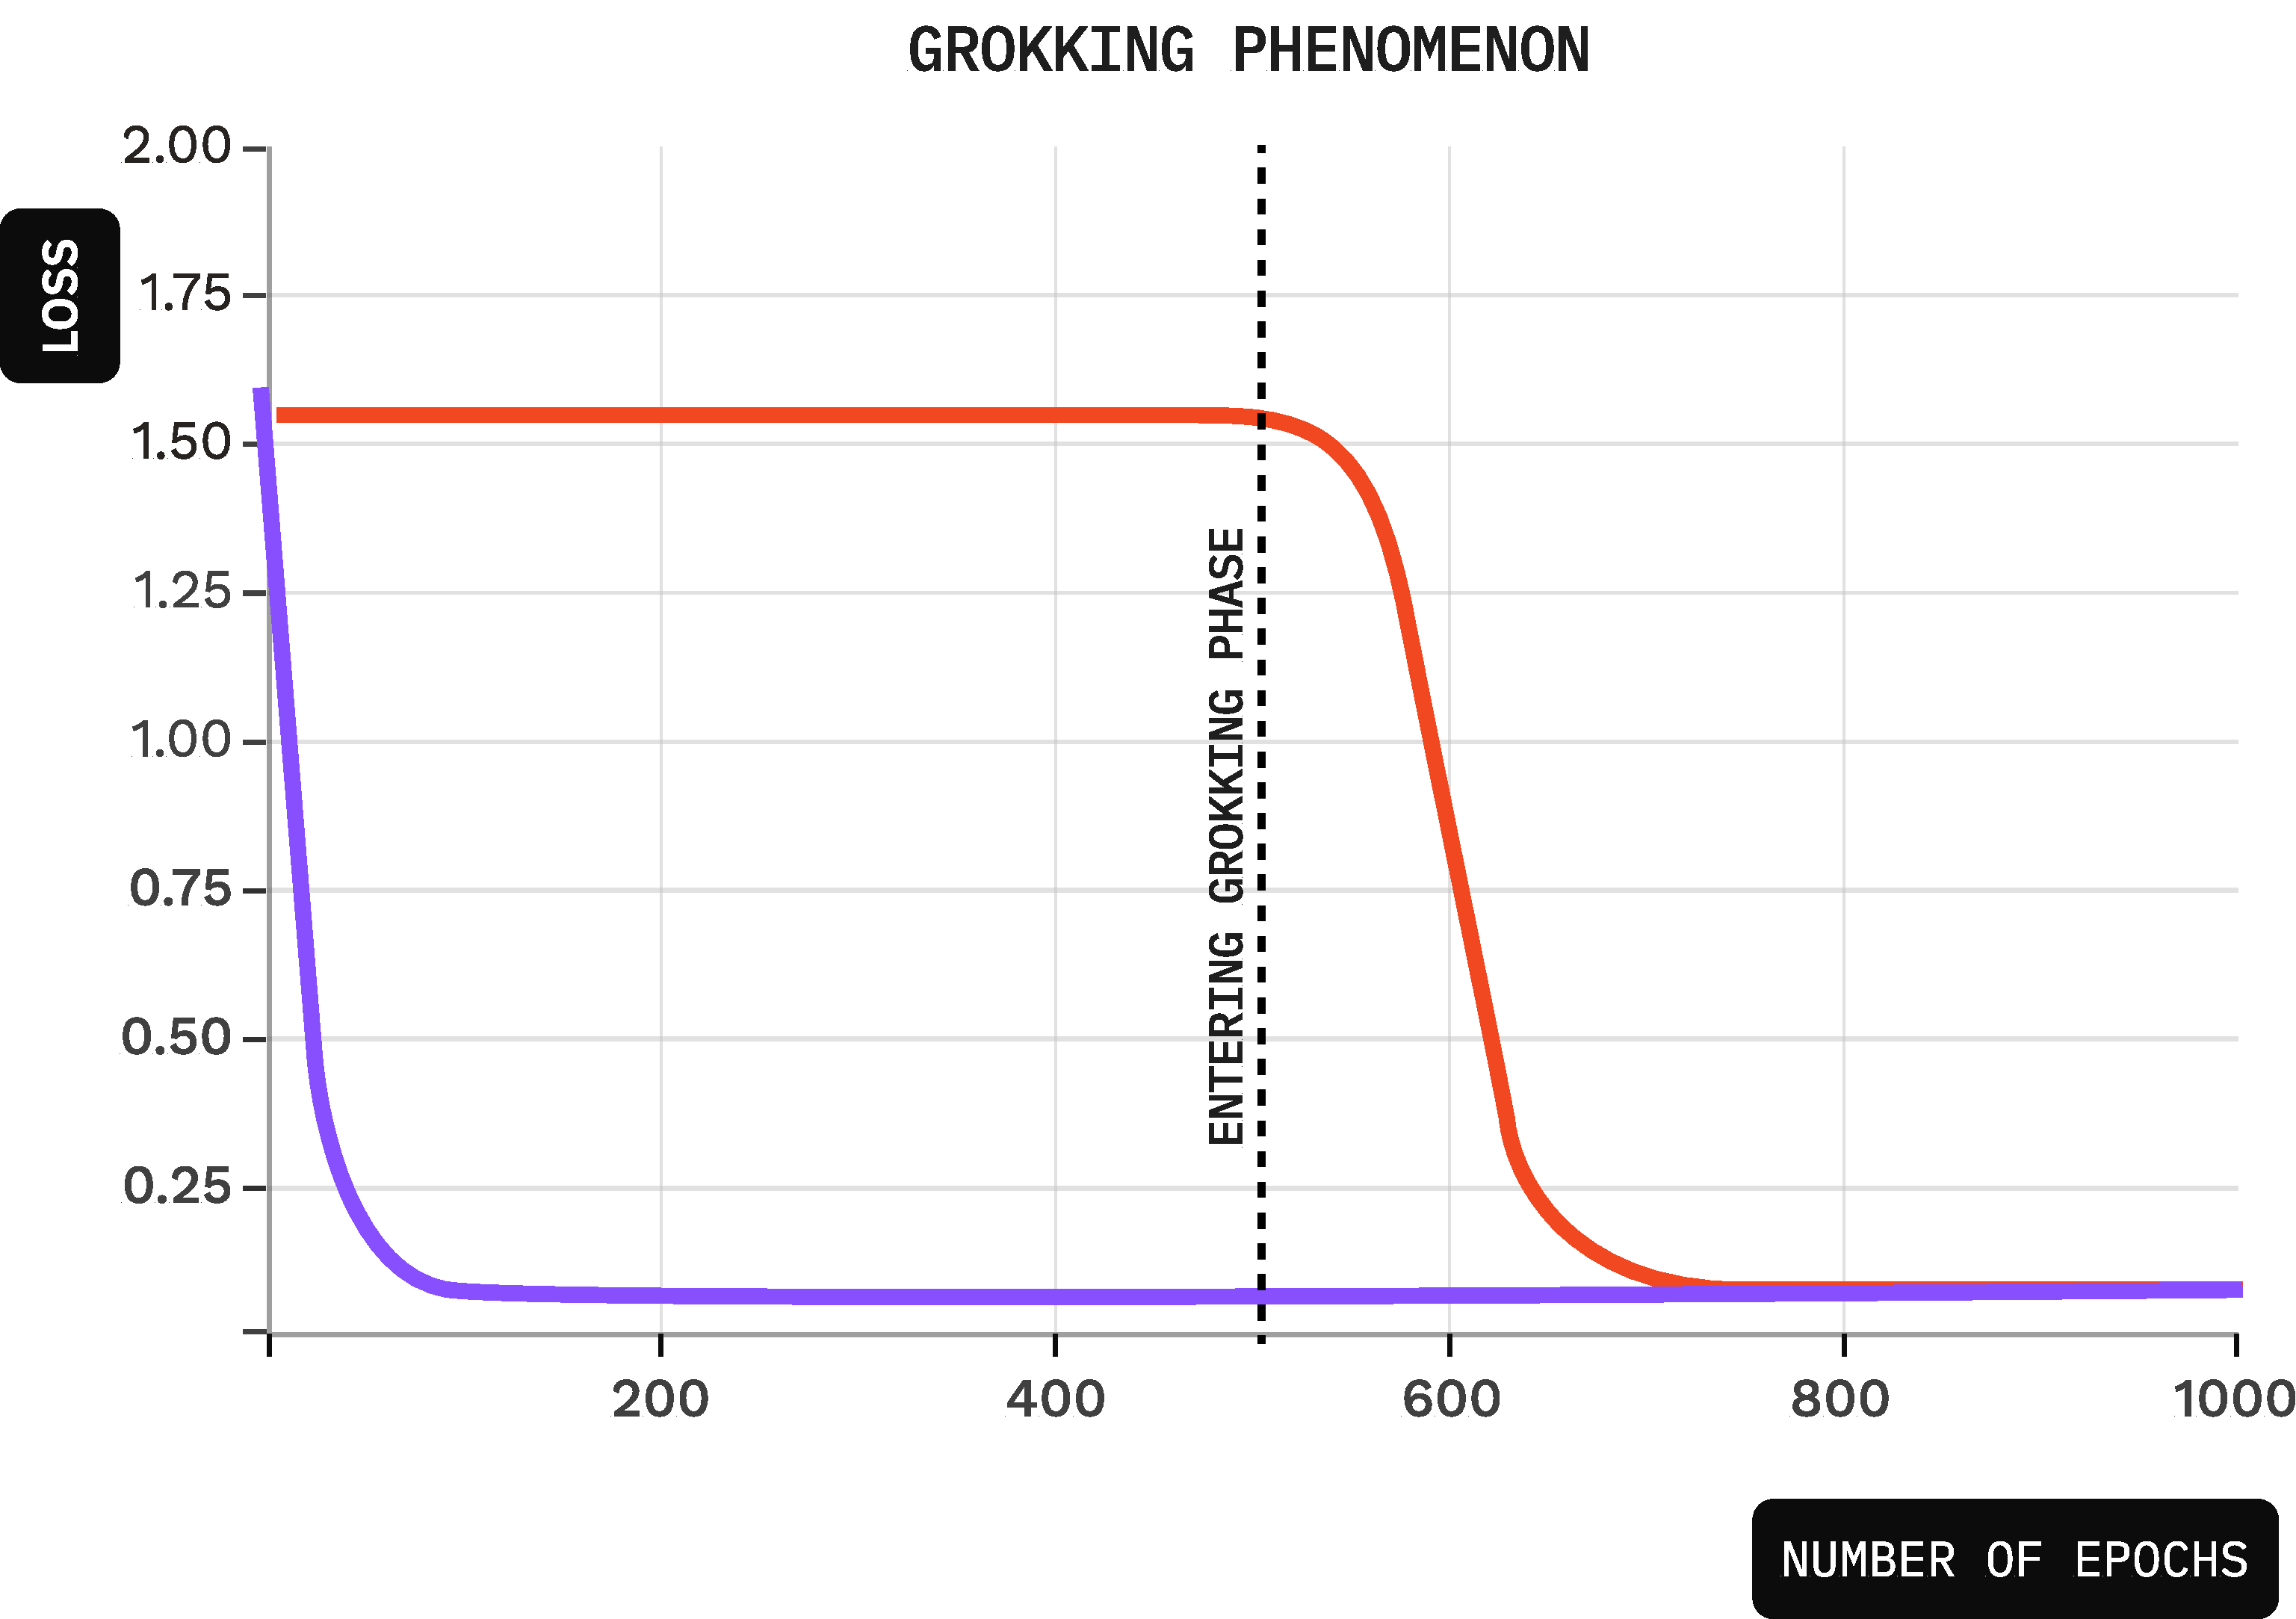
\includegraphics[width=0.8\linewidth]{figs/9_Grokking.pdf}
   \caption{\textbf{Grokking.} Training loss (purple) falls early in training while test loss (red) remains high. After a long plateau, test loss drops sharply, and the model generalises. Progress measures defined on model internals show the generalising circuit forming gradually during the plateau, before the change is visible in behaviour.}
   \label{fig:grokking}
\end{figure}

In modular arithmetic, training accuracy saturates early while test accuracy remains near chance for many steps before rising sharply (Figure~\ref{fig:grokking}; \citeemalp{power2022grokkinggeneralizationoverfittingsmall}). Mechanistic analysis of grokked networks recovers the learned algorithm (trigonometric identities implementing modular addition) and defines progress measures that track its formation: the generalising circuit grows gradually during the plateau, and the sharp change in test accuracy corresponds to a transition from a memorising solution to the completed generalising circuit followed by removal of the memorising components~\citeest{nanda2023progressmeasuresgrokkingmechanistic}. Grokking has been explained as competition between a memorising and a generalising circuit with different efficiencies under weight decay, an account that predicted and confirmed ungrokking and semi-grokking~\citeem{varma2023explaining}. Grokking can be induced or eliminated by controlling parameter norm at initialisation, and it occurs beyond algorithmic tasks~\citeest{liu2023omnigrok}.

\begin{warningbox}[Transfer from Grokking Settings to Language Models]
The standard setting in grokking experiments differs from language model pretraining in many ways, including dataset size, weight decay, and the number of epochs over the data. Current studies have not shown that existing quantitative conclusions transfer directly to large-scale pretraining.
\end{warningbox}

Similar findings have been reported outside grokking settings. \citetest{chen_sudden_2024} found that syntactic attention structures emerged during a sharp drop in masked language modelling (MLM) loss, before accuracy improvement on a grammatical benchmark. Similarly, \citetem{zucchet2025language} observed that attention-based recall circuits formed during a plateau in factual-knowledge acquisition, followed by rapid improvements in model performance. These findings suggest that changes in internal mechanisms can precede changes in model capabilities. This observation motivates research on forecasting model behaviour through internal monitoring, as discussed in Section~\ref{sec:ld-safety}.

\subsubsection{Attributing Transitions to Components}
\label{sec:ld-attribution}

So far, the methods we discussed cannot attribute the transition to specific model components. Attention head specialisation is probably the most intuitive option to work at this granularity in transformers. Individual attention heads can specialise to attend to syntactic relations, positional offsets, or rare tokens~(\citeestalp{voita_analyzing_2019}; \citeemalp{clark2019what}), and this specialisation can appear abruptly. For example, induction heads form during a brief training window, and their formation coincides with a sharp improvement in in-context learning~\citeem{olsson2022incontextlearninginductionheads}, a transition we examine in detail in Section~\ref{sec:ld-induction-case}. In masked language models, suppressing the syntactic attention structure delays the capability it precedes~\citeest{chen_sudden_2024}. Likewise, sparse attention emerges abruptly and depends on repetition in the training data~\citeest{zucchet2025the}.

These events cluster in time. Several attention heads, such as induction heads and heads exhibiting syntactic attention patterns, can acquire specialised functions within the same training window. These heads emerge alongside a peak in how accurately the model's perplexity predicts human reading times, and this predictive ability subsequently declines even as language modelling performance continues to improve~\citeest{aoyama_language_2025}. Head specialisation can be viewed as a form of \emph{symmetry breaking}. Before or in the very early stages of training, attention heads are indistinguishable and interchangeable; during training, they start to develop distinct functions despite having equivalent roles in the architecture. Tracking this process can help identify the emergence of modular structure. Attribution of this kind is also a diagnostic for modularity more broadly. Three observable indicators jointly diagnose modular internal structure~\citeem{zhao2024distributional}: transitions during training, emergent trends across model scale, and heterogeneous clustering of solutions across random seeds. A structure exhibiting all three is a strong candidate for a discrete, functionally specialised mechanism.



\begin{insightbox}[Sharp Transitions from Smooth Components]
Phase transitions in test loss or task accuracy do not imply abrupt change in any individual component. For example, in controlled settings, many attention heads develop induction-like behaviour gradually---their contributions are largely additive, and the sharp macroscopic transition arises from their aggregate effect~\citeest{singh2024needsrightinductionhead}. Localising a phase transition in a coarse-grained metric therefore does not help identify the responsible components. In contrast, component-level attribution may find only gradual change without being wrong.
\end{insightbox}

\subsubsection{Why Transitions Happen}\label{sec:training_phase_why}

\paragraph{Saddle-to-Saddle Dynamics.} Theoretical studies of deep linear networks show that different singular modes of the input--output correlations can be learned at different rates~\citeest{saxe2014exact,saxe2019mathematical}. The training process may therefore involve periods of slow improvement followed by rapid reductions in test loss. From an optimisation perspective, gradient descent moves through regions near successive saddle points in the loss landscape and gradually learns more complex solutions along the way. This process is known as \emph{saddle-to-saddle dynamics}. Similar training patterns have been observed in other neural networks, where they learn simpler functions before more complex ones~\citeest{rahaman2019spectral,nakkiran2019sgd}. Attention head specialisation may also be related to symmetry breaking during training, although the relationship to saddle-to-saddle dynamics is not yet fully established in realistic transformers~\citeest{chen_sudden_2024}.

\paragraph{Singular Learning Theory.} Singular learning theory (SLT) studies how the geometry of a singular model's parameter space affects learning and generalisation~\citeest{watanabe2009algebraic}. Neural networks are singular (and are thus a subject of study in SLT) because different parameter configurations can implement the same function. As a result, two models that achieve similar loss can differ substantially in their effective complexity. SLT provides a framework for studying this complexity and has motivated research on its changes during training and its usefulness in downstream applications~\citeest{lau2023local}.

\begin{definitionbox}[Local Learning Coefficient (LLC)]
For model parameters $\mathbf{\theta}^*$ at a local minimum, the Local Learning Coefficient (LLC) $\lambda(\mathbf{\theta}^*)$ measures the degeneracy of the loss landscape near $\mathbf{\theta}^*$ via the volume-scaling rate of low-loss neighbourhoods~\citeest{lau2023local}. Smaller values indicate more degenerate (flatter, in a higher-order sense) minima. The LLC is estimable at scale with stochastic-gradient MCMC~\citeest{lau2023local}.
\end{definitionbox}

Estimated LLC trajectories in transformers change at points that coincide with identifiable developmental events, including the stages of structure formation described in Section~\ref{sec:ld-attribution}~\citeest{hoogland2025losslandscapedegeneracystagewise}. This is the central empirical result of the developmental interpretability programme~\citeem{hoogland2023towards} introduced in Section~\ref{subsec:dev interp}. However, current evidence for LLC is largely retrospective, where phase transitions are detected and matched to known events only after training. Prospective prediction of a transition before it occurs has not yet been demonstrated. Section~\ref{sec:ld-safety} discusses potential applications of learning-dynamics analysis to forecasting and intervention.

\subsubsection{Case Study: Induction Heads}
\label{sec:ld-induction-case}

\begin{examplebox}[Learning Dynamics Perspective on Induction Heads]
The preceding case studies (Sections~\ref{subsec: induc head case study: feature extract} and \ref{subsec: induc head case study: circuit}) analysed induction heads and circuits in a trained model. Several facts about the induction circuit are invisible from that vantage point but become observable when we examine the model across training~\citeem{olsson2022incontextlearninginductionheads}. Consider the repeated sequence again

\[
\texttt{A B C A B \underline{?}},
\]

and observe at successive checkpoints of a single training run. Examining the checkpoints shows that the induction ability arrived abruptly: at early checkpoints the model bases its predictions on token frequencies and derives no benefit from the earlier occurrence of \texttt{A B}, and during a narrow window of training, roughly 2.5 to 5 billion tokens in the models studied by \citetem{olsson2022incontextlearninginductionheads}, induction heads form and the model begins predicting \texttt{C} by attending back to the first occurrence. A sharp improvement in in-context learning and a small bump in the training loss fall within the same window.\\

The timing of formation also helps provide causal evidence that a single model checkpoint cannot provide. Ablating an induction head in the final model only shows its necessity for the behaviour at that checkpoint. This does not support the stronger claim that the induction circuit's formation caused the capability to develop. \citetem{olsson2022incontextlearninginductionheads} examined this stronger claim by intervening on formation itself. Their ``smeared key'' modification built the previous-token head's contribution into the attention computation, allowing the circuit to form within a single layer. Under this modification, one-layer models acquire in-context learning they otherwise never develop, while the transition moves earlier in deeper models.
\end{examplebox}

\subsection{Leveraging Learning Dynamics for Safety}
\label{sec:ld-safety}
The analyses above also support safety-oriented objectives, including anticipating capabilities before they appear (Section~\ref{sec:ld-forecasting}) and intervening in the training process while it is still underway (Section~\ref{sec:ld-intervening}).

\subsubsection{Forecasting Model Behaviours}
\label{sec:ld-forecasting}

\paragraph{Forecasting from Smaller Runs and Partial Runs.} Scaling laws demonstrate that aggregate loss is predictable before training~(\citeemalp{kaplan2020scaling}; \citeestalp{hoffmann2022training}), but phase transitions break this style of extrapolation for individual capabilities (Section~\ref{sec:ld-transitions}). Forecasting therefore targets specific behaviours directly. Memorisation is the behaviour for which the forecasting problem has been posed most explicitly. \citetest{biderman2023emergent} introduced the problem of forecasting whether a specific training sequence will be memorised by a model before that model is trained. They argued that recall is the metric to optimise (a false negative means training a full model that leaks the sequence, while a false positive only discards a cheap trial run). They established baselines that forecast from smaller fully trained models and from partially trained checkpoints of the target run, together with equi-compute recommendations for dividing a fixed forecasting budget between model size and tokens.

\paragraph{Forecasting Safety-Relevant Behaviours.}
Emergence can be forecast by intervening on the training trajectory. Fine-tuning on a target task shifts capability emergence towards less capable models. Fitting how this shift varies with the amount of fine-tuning data yields an \emph{emergence law}. Using only small models, this law predicts whether a capability will have emerged in models trained with up to 4$\times$ more compute~\citeem{snell2024predicting}.

Rare harmful behaviours can also be forecast statistically. The largest elicitation probabilities observed in a small sample of queries scale predictably with query volume. This relationship allows harmful-behaviour risks to be extrapolated across up to three orders of magnitude of deployment-scale query volume. Examples include assisting with dangerous chemical synthesis and taking power-seeking actions~\citeem{jones2025forecasting}.

Post-training failures can be analysed similarly. Specifically, transitions between successive RLHF checkpoints can be classified into four categories: reward hacking, collapse, proxy under-alignment, and evaluator-specific disagreement. Reward hacking occurs when the model exploits a way to achieve high rewards while the external quality from the perspective of human users falls; collapse occurs when both decline. This classification localises failures that checkpoint averages miss. A model fitted to training-dynamics diagnostics predicts future reward hacking with a ROC-AUC of 0.82. These diagnostics include reward-model uncertainty, policy drift, and output diversity~\citeem{abahana2026rlhf}.

Internal signals extend forecasting to fine-tuning outcomes. Activation-space persona features predict whether a fine-tuned model will exhibit emergent misalignment~\citeest{wang2026persona}. Signals available before fine-tuning begins also predict the resulting model’s alignment~\citeem{zhang2026whatshapes}. Section~\ref{subsec: iat} discusses the research agenda these results instantiate.

\paragraph{Internal Precursors as Early Warning.} Where a mechanism forms before the capability it supports is behaviourally expressed, monitoring internals can flag the capability earlier than behavioural evaluation. The recall circuits that precede factual-knowledge acquisition~\citeem{zucchet2025language} and the syntactic attention structure that precedes the break in grammatical capabilities~\citeest{chen_sudden_2024} show that this lead time can exist; progress measures (Section~\ref{sec:ld-progress}) are the instrument that would exploit it.

\paragraph{Run-to-Run Variance.} To assess the reliability of a forecast, researchers can compare training runs with different random seeds. \citetest{vanderwal2025polypythias} found that capabilities generally emerge at similar stages and representations develop consistently across training runs, although some runs differ substantially. These exceptions highlight the uncertainty of forecasts based on a single training run.

\begin{warningbox}[Most Early-Warning Evidence Is Retrospective]
Currently, nearly all demonstrations that changes in internals lead to changes in behaviour are retrospective. In these studies, researchers analyse the completed mechanism after training to identify a progress measure or precursor structure, then evaluate it backwards over saved checkpoints. This concern also exists in LLC-based transition detection (Section~\ref{sec:training_phase_why}).\\

In contrast, prospective forecasting requires researchers to predict outcomes before observing them. \citetest{biderman2023emergent} proposed baseline methods for forecasting memorisation. However, prospective forecasting for broader capability transitions relevant to AI safety remains underdeveloped. Early-warning signals therefore require prospective validation before they can be considered reliable.

\end{warningbox}

\subsubsection{Intervening on Training Processes}
\label{sec:ld-intervening}

The model that matters is the one deployed at the end of training, and the standard response to an undesirable behaviour found there is post-training fine-tuning, which is outside the scope of this section. An alternative is to intervene during training to prevent undesirable capabilities from developing or to control how they develop. Existing work explores three approaches: modifying training data, changing model architecture, and intervening on model activations during fine-tuning.

\paragraph{Pretraining Data Filtering: Deep Ignorance.} Deep Ignorance filters proxies for biohazardous knowledge out of the pretraining corpus and trains 6.9-billion-parameter models on the filtered data (Section~\ref{sec:ld-data}; \citeestalp{obrien2026deep}). The filtered models do not acquire the targeted knowledge, making it difficult for the unwanted capability to emerge through adversarial fine-tuning. In contrast, post-training unlearning may suppress the unwanted behaviour without removing the underlying knowledge. A follow-up moves the filter from documents to tokens: individual tokens are labelled using sparse autoencoders and efficient classifiers trained on those labels, and filtering at token granularity removes the undesired capability at lower cost to desired capabilities than document-level filtering, with effectiveness increasing with model scale across the two orders of magnitude tested and filtered models remaining alignable afterwards~\citeem{rathi2026shaping}.

Similarly, the order in which different categories of training data are presented matters. \citetem{bruijns2026pretrainingcurriculaenableselective} found that, in an imbalanced pretraining curriculum where one task is shown before another, the model packs the tasks sequentially into separable circuits, resulting in more targeted subsequent refusal fine-tuning.

\begin{warningbox}[Data-Level Interventions Have Ripple Effects]
Removing data from a training set does not act only on the removed data. In the setting of \citetest{borkar2025privacy}, deleting personal information can increase memorisation of the personal information that remains, and adding one individual's information amplifies memorisation of others' by roughly 7.5$\times$, because whether a sequence is memorised depends on similar sequences seen elsewhere in training. Subliminal learning~\citeest{cloud2026language} shows that data can transmit traits not apparent from its semantic content. For example, a student model can inherit a teacher's hidden bias from seemingly unrelated data, such as number sequences. This transfer is carried by a small set of divergence tokens and depends on early layers~\citeest{schrodi2026towards}. Filtering and unlearning interventions therefore need to be evaluated on what the model does with the data that stays, not only on what it no longer does with the data that was removed.
\end{warningbox}

\paragraph{Architectural Modification: Gradient Routing.} Gradient routing is an architectural modification informed by learning dynamics: it constrains which parameters receive gradient updates for chosen concepts during training, localising the corresponding computation into designated regions of the network~\citeem{cloud2024gradient}. Although the modification does not make the trained model safer on its own, it shapes where a mechanism forms so that later interventions, such as gating the designated region, become clean and localised. The antecedent for this style of intervention is the smeared-key modification~\citeem{olsson2022incontextlearninginductionheads}, which showed that an architectural change can control when and whether a mechanism forms at all (Section~\ref{sec:ld-induction-case}).

\paragraph{Monitoring and Steering During Fine-Tuning.} The case excluded above uses fine-tuning to repair an undesirable behaviour after it has been identified. Intervening on the fine-tuning process itself remains within scope, and persona vectors provide a current example of this approach. A persona vector is an activation-space direction corresponding to a character trait such as sycophancy, hallucination propensity, or malice, extractable automatically from a natural-language trait description~\citeem{chen2025persona}. Intended and unintended personality changes during fine-tuning correlate strongly with movement along the relevant vector, which yields the monitoring instrument. Preventative steering along the vector during fine-tuning limits acquisition of the trait. Before fine-tuning, projecting training data onto the vector flags data that would induce the trait, at both the dataset and individual-sample levels~\citeem{chen2025persona}. This instantiates each step of the intervention loop below for the fine-tuning stage.

\begin{practicebox}[Train-Time Intervention Loop]
The work discussed so far lays the methodological foundation for intervening in a training run in progress. Below we present a general pipeline.

\begin{enumerate}[nosep]
   \item \textbf{Monitor} a target quantity at checkpoints, such as a capability-specific metric (Section~\ref{sec:ld-detect}) or a progress measure on model internals (Section~\ref{sec:ld-progress}).
   \item \textbf{Define} the acceptable range for that quantity in advance, including the response to a breach.
   \item \textbf{Intervene} when the range is breached, such as by adjusting the data mixture or filtering out unwanted data, applying a targeted architectural or regularisation change, rolling back to a pre-breach checkpoint, and resuming under the adjusted setup.
   \item \textbf{Re-evaluate} the model after the intervention to verify that the targeted capability has been suppressed and does not re-emerge during further training.
\end{enumerate}
No published system implements this loop end to end at scale. Instead, existing studies have demonstrated individual steps of the proposed workflow.
\end{practicebox}

\paragraph{Open Questions.}
Three questions remain about the applicability of these training-time interventions. First, effective data filtering requires identifying which training data contributes to the capability we want to remove. Token-level filtering is motivated by data attribution, but it remains unclear whether methods such as influence functions (Section~\ref{sec:influence-functions}) can reliably identify the relevant data. Second, scale: Deep Ignorance operates at 6.9 billion parameters, and while token-level filtering became more effective across the tested scale range~\citeem{rathi2026shaping}, it remains open whether data filtering stays effective and affordable at frontier scale. Third, deployed models show that stronger train-time safeguards are achievable, but not how: gpt-oss models are substantially harder to fine-tune than comparable open-weight models, and their developers have not fully disclosed their responsible training procedure~\citeem{openai2025gptoss120bgptoss20bmodel}. Understanding how this resistance is achieved could help develop similar safeguards for other open-weight models and clarify how fine-tuning changes model behaviour.

\paragraph{Summary.}
Learning dynamics can be studied both as an object of explanation, revealing how representations and mechanisms evolve during training, and as an interpretability tool to localise mechanisms, detect phase transitions, and test causal hypotheses through training interventions. Understanding learning dynamics can also help predict when capabilities emerge and guide interventions during training. However, no complete system combining monitoring and intervention has yet been demonstrated at scale. This section focuses on how models change during training, while Section~\ref{sec:influence-functions} examines how individual training examples contribute to model behaviour.
